\documentclass[11pt,letterpaper]{article}
\usepackage{graphicx, geometry, amsmath, hyperref, url, natbib, booktabs, longtable, xcolor}
\geometry{margin=1in}
\hypersetup{colorlinks=true, linkcolor=black, citecolor=black, urlcolor=black}
\renewcommand{\topfraction}{0.9}
\renewcommand{\bottomfraction}{0.8}
\renewcommand{\textfraction}{0.07}
\renewcommand{\floatpagefraction}{0.75}

\title{Sharpness-Aware Minimization and Test NLL Beyond Temperature Scaling on Fashion-MNIST}
\author{}
\date{}

\begin{document}
\maketitle

\begin{abstract}
On a small convolutional network trained on Fashion-MNIST, sharpness-aware minimization (SAM) has a lower test negative log-likelihood (NLL) than validation-tuned stochastic gradient descent (SGD) after both models are temperature-scaled: 0.033 lower in NLL (95\% CI $-0.040$ to $-0.026$; Holm-corrected $p = 0.0018$). This is a single estimate from one tuned comparison over five paired seeds on the test set, a lead rather than a confirmed result, not specified in advance and not reproduced in an independent study. The scope is one dataset, one small architecture and five seeds. A shuffled-label control produces a larger NLL gap than the real comparison, so the advantage reflects how confident the models are rather than learned label information. SAM's lower raw expected calibration error (ECE) does not remain once SGD is temperature-scaled, and SAM's accuracy is higher at the tuned SGD learning rate, though not at a learning rate of 0.01. SAM updates parameters with the gradient taken at a worst-case point within a small radius of the current weights. Tan et al. report that it counteracts overconfidence, with a comparison against temperature-scaled SGD on ResNet-56. Learning rates and the SAM radius were tuned on validation NLL with a separate seed. Two smaller studies, with weaker baselines or at matched training loss, point the same way and are reported as supporting evidence, not pooled with the main result.
\end{abstract}

\section{Introduction}
Classifiers trained with cross-entropy often assign confidence above their accuracy on held-out data, and temperature scaling, a single fitted scalar, is a common post-hoc fix \citep{Guo2017}. Calibration matters where a confidence value is acted on, as in medical diagnosis and driving, and the usual summary, expected calibration error (ECE), can fail to reveal miscalibration \citep{Nixon2019}.

Sharpness-aware minimization (SAM) changes the training update rather than the output layer. It computes the gradient at the point within a small radius of the current weights where the loss is highest, and it steps with that gradient \citep{Foret2020}. \citet{Tan2026} argue that SAM counteracts overconfidence and compare SAM with temperature-scaled SGD on ResNet-56. A 2026 preprint reports that calibration error follows the curvature of the loss \citep{Morosini2026}. The comparisons in these studies do not always tune the SGD baseline as carefully as SAM, and a calibration gain can come from a global shift in confidence, which a single-parameter rescaling would also produce. The question this paper addresses is specific: on a small convolutional network, does SAM outperform a learning-rate-tuned SGD on calibration once the SGD baseline is given the same temperature scaling?

We tune both optimisers on validation NLL, train each with five paired seeds, and compare SAM with SGD and with temperature-scaled SGD (TS-SGD). The contributions are:

\begin{itemize}
  \item SAM has a lower test NLL than validation-tuned SGD after both models are temperature-scaled, by 0.033 in NLL (95\% CI $-0.040$ to $-0.026$, Holm-corrected $p = 0.0018$). This is a lead: one tuned comparison over five paired seeds, not specified in advance and not reproduced in an independent study (Section~\ref{sec:nll}).
  \item The raw ECE advantage of SAM over SGD ($-0.0050$, 95\% CI $-0.0079$ to $-0.0021$) does not remain after temperature scaling of SGD. There the difference is $+0.0020$, with an interval that includes zero (Section~\ref{sec:ece}).
  \item SAM's test accuracy is higher at the validation-tuned SGD learning rate, by 0.96 points. At a learning rate of 0.01 the accuracy difference does not differ from zero (Section~\ref{sec:acc}).
  \item A shuffled-label control produces an NLL gap larger than the real one, so the NLL advantage cannot be attributed to label information (Section~\ref{sec:nll}).
\end{itemize}

Figure~\ref{fig:headline} shows the primary contrasts with their 95\% intervals. Section~\ref{sec:related} reviews related work, Section~\ref{sec:method} describes the method and protocol, Section~\ref{sec:results} reports results, and Sections~\ref{sec:discussion} to~\ref{sec:conclusion} discuss, limit and conclude.

\begin{figure}[!htbp]
  \centering
  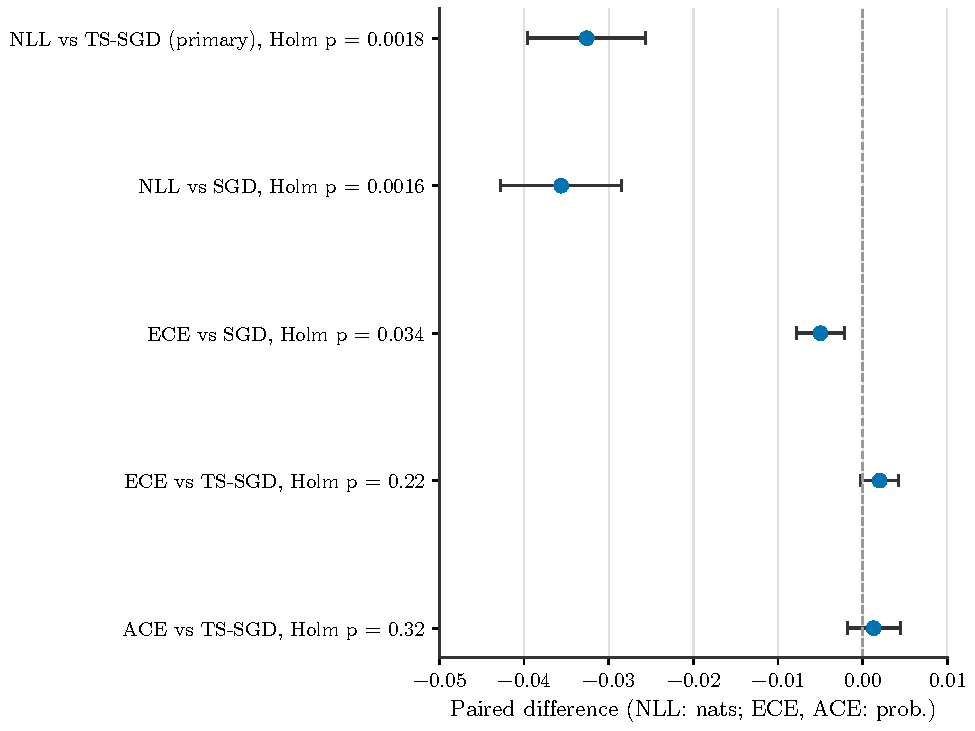
\includegraphics[width=\linewidth,height=0.45\textheight,keepaspectratio]{figures/fig2_v0.pdf}
  \caption{Paired differences, SAM minus baseline, across five seeds with 95\% paired t-intervals; Holm-adjusted p-values are shown per row. The NLL contrast against temperature-scaled SGD (TS-SGD, primary row) excludes zero; ECE against unscaled SGD does too, but ECE and ACE against TS-SGD do not. One tuned estimate: a lead, not a confirmed finding.}
  \label{fig:headline}
\end{figure}

\section{Related Work}\label{sec:related}
\textbf{Calibration and post-hoc correction.} \citet{Guo2017} measured the calibration of modern networks, found that depth, width, weight decay and batch normalisation affect it, and showed that temperature scaling is an effective post-hoc correction. \citet{Nixon2019} showed that ECE can read as low for a poorly calibrated model, because binning hides errors, and they argued for complementary metrics. This paper keeps ECE with equal-width bins so that results are comparable with that literature, and it adds NLL, a proper scoring rule, and a temperature-scaled SGD control. The difference is that the control is an analysis step, not a correction reported once.

\textbf{Sharpness and calibration.} SAM \citep{Foret2020} replaces the loss at the current weights with a worst-case loss inside a small neighborhood. \citet{Tan2026} link SAM to lower overconfidence through an implicit entropy effect and compare it with temperature-scaled SGD on ResNet-56, so the temperature control is not new here; the new scope is a small network, the NLL metric and a matched-loss design. \citet{Morosini2026} link calibration to curvature. This work differs by tuning the SGD learning rate on validation NLL, by reporting the paired contrast against temperature-scaled SGD, and by checking the NLL result against a shuffled-label control. It uses a small network on Fashion-MNIST \citep{Xiao2017}, where many seeds and several learning rates can be run.

\section{Method}\label{sec:method}
\textbf{Optimisers.} SGD uses momentum 0.9 on mini-batches. SAM with radius $\rho$ computes the gradient $g$ at the current weights $w$, moves to $w + \rho\, g/\lVert g\rVert$, computes the gradient there, and applies that gradient to $w$ \citep{Foret2020}. Both optimisers share the architecture, batch size, weight decay, cosine learning-rate schedule and epoch count, and both use the same initialisation and batch order for each seed.

\textbf{Data and model.} Fashion-MNIST \citep{Xiao2017} has 60,000 gray 28 by 28 images in 10 fashion classes. We split its training images into 50,000 for training and 10,000 for validation, and we evaluate each final model once on the standard 10,000-image test set. The network has two convolutional blocks, each with batch normalisation and 2 by 2 max pooling, followed by two linear layers.

\textbf{Tuning protocol.} Learning rates and the SAM radius are chosen on tuning seed 101 by the lowest final validation NLL. The grid is SGD learning rate in $\{0.0003, 0.001, 0.003, 0.01, 0.03\}$, SAM learning rate in $\{0.001, 0.003, 0.01, 0.03\}$ and SAM radius in $\{0.05, 0.1, 0.2\}$. The selected settings are SGD at learning rate 0.001 (validation NLL 0.214) and SAM at learning rate 0.01 with radius 0.1 (validation NLL 0.182). Neither selected value lies on an edge of its grid, and the test set plays no part in selection. Final results use seeds 0 to 4, which differ from the tuning seed.

\textbf{Calibration metrics and temperature scaling.} Confidence is the top-label softmax probability. ECE is the bin-weighted average absolute gap between accuracy and confidence over 15 equal-width bins. Adaptive calibration error (ACE) is the same average over equal-mass bins, and NLL is the mean negative log probability of the true class. For the control, we fit a single temperature $T$ that divides the logits and minimises validation NLL, and we apply it unchanged to the test logits. We report temperatures for both optimisers to show the direction of any miscalibration.

\textbf{Statistics.} For each seed we take the difference between two groups, then report the mean difference with a 95\% paired t-interval (df = 4) and a two-sided p-value. The 12-row family in Table~\ref{tab:main} is corrected with Holm's step-down procedure. The shuffled-label control shuffles the test labels and runs the same pipeline.

\section{Results}\label{sec:results}
\subsection{SAM lowers test NLL against temperature-scaled SGD}\label{sec:nll}
Table~\ref{tab:main} reports the primary family. The result is a lead, meaning one estimate from one tuned comparison: it was run once after tuning, it was not specified in advance, and it has not been reproduced in an independent study. The NLL difference against temperature-scaled SGD is $-0.0326$ in NLL, with interval $-0.0396$ to $-0.0256$ and Holm-corrected $p = 0.0018$. Every seed shows a negative difference, between $-0.025$ and $-0.041$. Raw NLL is lower still ($-0.0356$), so temperature scaling removes part of the gap, but about 0.033 in NLL remain once both models are scaled. Figure~\ref{fig:headline} plots these contrasts, and Figure~\ref{fig:seeds} shows the seed-level differences.

\begin{table}[!htbp]
  \centering
  \caption{Paired differences, SAM minus baseline, five seeds (0 to 4), test set. Intervals are 95\% paired t-intervals (df = 4). Holm p is corrected across the 12-row family.}
  \label{tab:main}
  \begin{tabular}{llrrr}
    \toprule
    Contrast & Metric & Mean difference & 95\% CI & Holm p \\
    \midrule
    SAM minus SGD & Accuracy (points) & +0.96 & +0.65 to +1.27 & 0.007 \\
    SAM minus SGD & ECE & $-0.0050$ & $-0.0079$ to $-0.0021$ & 0.034 \\
    SAM minus SGD & NLL & $-0.0356$ & $-0.0427$ to $-0.0285$ & 0.0016 \\
    SAM minus TS-SGD & ECE & $+0.0020$ & $-0.0003$ to $+0.0043$ & 0.22 \\
    SAM minus TS-SGD & ACE & $+0.0013$ & $-0.0019$ to $+0.0044$ & 0.32 \\
    SAM minus TS-SGD & NLL & $-0.0326$ & $-0.0396$ to $-0.0256$ & 0.0018 \\
    \bottomrule
  \end{tabular}
\end{table}

\begin{figure}[!htbp]
  \centering
  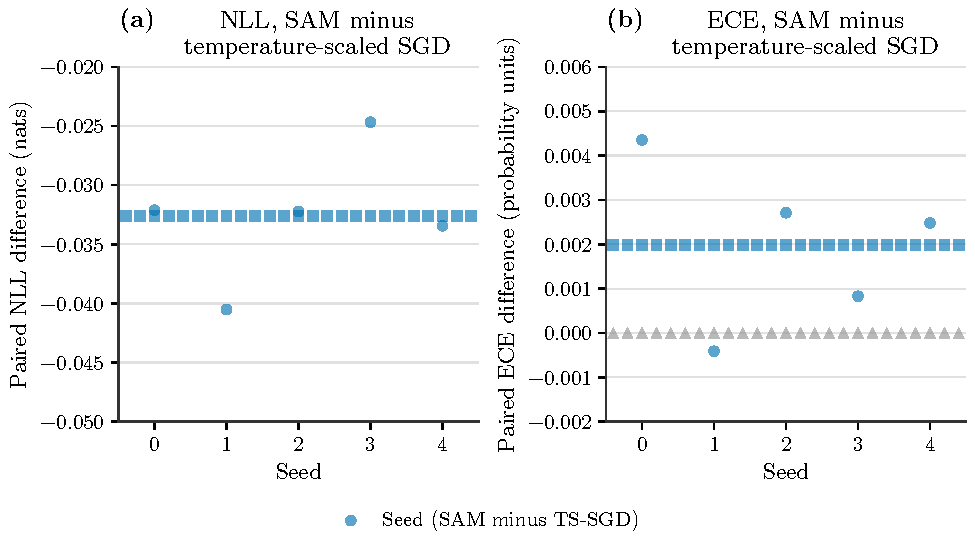
\includegraphics[width=\linewidth,height=0.45\textheight,keepaspectratio]{figures/fig3_v0.pdf}
  \caption{Paired SAM minus temperature-scaled SGD differences for five seeds (0--4); blue dots are seeds and blue squares the mean across seeds. Every seed gives lower NLL for SAM, while the ECE differences cross zero (gray markers show zero in (b) only).}
  \label{fig:seeds}
\end{figure}

The shuffled-label control limits this result. When the test labels are shuffled, the raw SAM-minus-SGD NLL difference is $-0.224$ (two-sided $p = 0.009$), which is larger in magnitude than the real raw difference of $-0.036$. NLL responds to how confident a model is, and a lower-confidence model scores better on shuffled labels, so the NLL advantage is not evidence that SAM learns more label structure. Accuracy does not respond to the shuffle (shuffled-label control difference $-0.0003$).

\subsection{The raw ECE advantage is a confidence-scale effect}\label{sec:ece}
Raw SAM has a lower ECE than raw SGD ($-0.0050$, Holm $p = 0.034$). The fitted temperatures explain it. SGD has a mean temperature of 1.05 (range 1.03 to 1.06 across seeds), so raw SGD is overconfident, while SAM has a mean of 0.94 (range 0.92 to 0.95), so raw SAM is slightly underconfident. Once SGD is scaled, the ECE difference is $+0.0020$ (interval $-0.0003$ to $+0.0043$, Holm $p = 0.22$), and the ACE difference is $+0.0013$ (interval $-0.0019$ to $+0.0044$). The calibrated ECE advantage that the raw comparison suggests is therefore not supported in this design.

At this learning rate SAM also reaches a lower final training loss than SGD (mean 0.110 against 0.122). The fit gap that complicates the first 40-epoch design, where SAM was under-fitted, does not apply to this tuned comparison.

\subsection{Accuracy and the matched checks}\label{sec:acc}
SAM's accuracy is 0.96 points higher than SGD at the validation-tuned learning rate (Table~\ref{tab:main}, Holm $p = 0.007$). The size of this difference depends on the SGD learning rate. In the 40-epoch design, where SGD used learning rate 0.01, the difference was 0.15 points and was not significant (Holm $p = 0.135$). Table~\ref{tab:supp} gathers the remaining checks, each of which uses its own design and is not pooled with Table~\ref{tab:main}.

\begin{table}[!htbp]
  \centering
  \caption{Supporting designs. Each row is a separate design with its own baseline, so the values are not pooled with Table~\ref{tab:main}.}
  \label{tab:supp}
  \footnotesize\raggedright
  \begin{tabular}{p{0.28\linewidth}p{0.08\linewidth}p{0.22\linewidth}p{0.30\linewidth}}
    \toprule
    Design & Seeds & Contrast & Mean difference (95\% CI) \\
    \midrule
    SGD at learning rate 0.01, 40 epochs & 5 & SAM minus TS-SGD, NLL & $-0.0196$ ($-0.0257$ to $-0.0136$) \\
    SGD at learning rate 0.01, 40 epochs & 5 & SAM minus SGD, raw ECE & $-0.0378$ ($-0.0414$ to $-0.0341$) \\
    SGD trained to SAM's training loss, 10 epochs & 5 & SAM minus TS-SGD, NLL & $-0.0082$ ($-0.0110$ to $-0.0053$) \\
    SGD trained to SAM's training loss, 10 epochs & 5 & SAM minus SGD, raw ECE & $-0.0076$ ($-0.0091$ to $-0.0061$) \\
    SGD at learning rate 0.03, 60 epochs & 3 & SAM minus SGD, ECE (descriptive) & $-0.017$ (no interval) \\
    \bottomrule
  \end{tabular}
\end{table}

At matched training loss, SAM's accuracy is 0.25 points higher than SGD's at learning rate 0.01 (Holm $p = 0.055$). Its NLL advantage over temperature-scaled SGD remains, smaller in size than in the 40-epoch design, which is consistent with part of that design's NLL gap being a fit effect.

\subsection{Training trajectories}\label{sec:traj}
In a separate design, three seed pairs were trained for 60 epochs at learning rate 0.03 without tuning. At epoch 60 the test ECE is 0.028 for SAM and 0.045 for SGD, and the NLL is 0.076 lower for SAM. Under temperature scaling the ECE gap falls to 0.007 against 0.009. At matched training loss, SAM's top Hessian eigenvalue is 12 to 16 lower and its validation ECE is 0.010 to 0.014 lower. These are point estimates from three seeds, and no p-values are reported.

An analysis of the same trajectories shows that the validation gap is near zero over epochs 1 to 5, reaches its largest mean advantage for SAM around epochs 25 to 30, and then falls after the peak, so the epoch-60 endpoint is not the maximum. Within one 40-epoch run, the test ECE gap is $-0.013$ at epoch 5 and $-0.038$ at epoch 40. The gap therefore grows with training in these trajectories, but the 60-epoch gap does not keep growing to the end.

\section{Discussion}\label{sec:discussion}
The NLL result is the one that remains under the controls in this setting. SAM has lower NLL than SGD in every design, and the NLL advantage remains after both models are temperature-scaled. Its size, however, depends on the SGD baseline: $-0.0326$ in NLL against the validation-tuned SGD, and $-0.0082$ against SGD matched to SAM's training loss at a learning rate of 0.01. A reader should expect a gain of this kind to fall when the baseline is stronger, and an evaluation that uses a weaker baseline will make it look larger.

The ECE result is a confidence-scale effect. Temperature scaling removes SAM's raw ECE advantage on this network, because the advantage comes from SGD's overconfidence, which a single scalar corrects. For evaluations of calibration methods, the implication is that a raw-confidence comparison against an unscaled baseline measures how much the baseline is overconfident, not whether the method ranks predictions better. Calibration claims should be reported against a temperature-scaled baseline.

The shuffled-label control result matters for the same reason. NLL and the Brier score respond to confidence level even when labels contain no information, so a shuffled-label control that passes for accuracy but fails for NLL is the expected pattern, not a sign of an error in the pipeline. An evaluation of a training method's calibration should include a shuffled-label check and report how far it moves the metric.

\section{Limitations}\label{sec:limitations}
The main result is a lead: one tuned estimate. It was not specified in advance, it has not been reproduced in an independent study, and the validation split serves both tuning and temperature fitting. The matched-fit check at the tuned SGD learning rate of 0.001 has not been run, so whether the NLL advantage holds at matched training loss at that rate is open. The tuning seed (101) is separate from the final seeds (0 to 4), and the test set is not used for selection, but no held-out test was run on new seeds.

Five paired seeds give low power. An exact sign-flip test cannot reach $p$ below 0.05 with five seeds (its smallest value is 0.0625), so the reported p-values rely on the t-approximation, and the intervals are wide.

The shuffled-label control shows that NLL and ECE respond to confidence level even without label information, so the NLL result does not isolate learned structure. We did not run a shuffled-label control against temperature-scaled SGD, so the shuffled-label control comparison is against raw SGD.

The matched-loss design used SGD at learning rate 0.01, which was the worst of the five SGD rates on validation NLL in the tuning grid (0.273 against 0.214 at the selected rate). Its NLL and ECE advantages are therefore against a weaker baseline than the primary result's. The trajectory design used three seeds, without tuning, and reports point estimates only. A 60-epoch extension of the 40-epoch design was not run.

The study covers one dataset and one small network. Results on larger models, such as those of \citet{Tan2026}, are not tested here.

\section{Conclusion}\label{sec:conclusion}
On a small convolutional network for Fashion-MNIST, SAM has a lower test NLL than a validation-tuned SGD after both models are temperature-scaled. The difference is 0.033 in NLL (95\% CI $-0.040$ to $-0.026$), a lead from one tuned estimate over five paired seeds, and a shuffled-label control shows that part of this NLL effect is a confidence effect rather than learned label information. SAM's lower raw ECE does not remain after temperature scaling of the baseline, and SAM's accuracy advantage depends on the SGD learning rate. Evaluations of SAM's calibration should use a tuned, temperature-scaled baseline and a shuffled-label control. Tests on larger networks and on new seeds would show whether the NLL gap holds beyond this setting.

\section*{Code and data}
Code and raw outputs that reproduce each number are in the paper's code~\href{https://github.com/ai-inventor-papers/ai-invention-d46016-sharpness-aware-training-makes-small/tree/main}{[code]}, and Appendix~\ref{app:code} links each result to the code path that produced it.

\clearpage
\bibliographystyle{plainnat}
\bibliography{references}

\clearpage
\appendix
\section{Task, inputs and scoring}
Each model takes one 28 by 28 gray image and outputs a probability vector over 10 fashion classes. An output is correct when its highest-probability class equals the image's label. Accuracy is the fraction of correct outputs. Confidence is the highest class probability. ECE uses 15 equal-width bins over confidence, and each bin contributes its share of examples times the absolute gap between its mean accuracy and its mean confidence. ACE uses equal-mass bins. NLL is the mean of minus the log probability assigned to the true class. The models take images as input, so no text input is given. Results use the standard 10,000-image test set, and temperature scaling uses only the 10,000 validation images.

\section{Experimental designs}
The primary tuned comparison is the one reported in Table~\ref{tab:main}. The 40-epoch design uses five seeds, 40 epochs, a learning rate of 0.01 for SGD (at the lower edge of its grid) and the tuned SAM setting. The 60-epoch design uses three seeds, 60 epochs and learning rate 0.03, with no tuning. The matched-loss design trains SGD for the number of epochs whose training loss matches SAM's 40-epoch loss within 0.01, at learning rate 0.01. Each design's artifact holds its full per-run records.

\section{Code for each result}\label{app:code}
Each row links the code path of the experiment behind a result.

\begin{longtable}{p{0.14\linewidth}p{0.50\linewidth}p{0.28\linewidth}}
  \toprule
  Section & Result & Code path \\
  \midrule
  \endhead
  \S\ref{sec:nll} & Primary NLL contrast against TS-SGD, Table~\ref{tab:main}, Figure~\ref{fig:headline}; shuffled-label control & \href{https://github.com/ai-inventor-papers/ai-invention-d46016-sharpness-aware-training-makes-small/tree/main/round-2/experiment-3}{\texttt{round-2/experiment-3}} \\
  \S\ref{sec:ece} & Raw and temperature-scaled ECE and ACE contrasts, Table~\ref{tab:main}; 40-epoch ECE gap by epoch & \href{https://github.com/ai-inventor-papers/ai-invention-d46016-sharpness-aware-training-makes-small/tree/main/round-2/experiment-3}{\texttt{round-2/experiment-3}}, \href{https://github.com/ai-inventor-papers/ai-invention-d46016-sharpness-aware-training-makes-small/tree/main/round-1/experiment-1}{\texttt{round-1/experiment-1}} \\
  \S\ref{sec:acc} & Accuracy at the tuned SGD rate, Table~\ref{tab:main}; accuracy at learning rate 0.01 and 40-epoch checks, Table~\ref{tab:supp} & \href{https://github.com/ai-inventor-papers/ai-invention-d46016-sharpness-aware-training-makes-small/tree/main/round-2/experiment-3}{\texttt{round-2/experiment-3}}, \href{https://github.com/ai-inventor-papers/ai-invention-d46016-sharpness-aware-training-makes-small/tree/main/round-1/experiment-1}{\texttt{round-1/experiment-1}} \\
  \S\ref{sec:acc} & Matched-loss accuracy and NLL checks, Table~\ref{tab:supp}, Figure~\ref{fig:seeds} & \href{https://github.com/ai-inventor-papers/ai-invention-d46016-sharpness-aware-training-makes-small/tree/main/round-2/experiment-4}{\texttt{round-2/experiment-4}} \\
  \S\ref{sec:traj} & Training trajectories of the 60-epoch design & \href{https://github.com/ai-inventor-papers/ai-invention-d46016-sharpness-aware-training-makes-small/tree/main/round-1/experiment-2}{\texttt{round-1/experiment-2}} \\
  \S\ref{sec:traj} & Validation-gap analysis of the trajectories & \href{https://github.com/ai-inventor-papers/ai-invention-d46016-sharpness-aware-training-makes-small/tree/main/round-2/evaluation-1}{\texttt{round-2/evaluation-1}} \\
  \bottomrule
\end{longtable}

\end{document}
